%%%%%%%%%%%%%%%%%%%% author.tex %%%%%%%%%%%%%%%%%%%%%%%%%%%%%%%%%%%
%
% sample root file for your "contribution" to a contributed volume
%
% Use this file as a template for your own input.
%
%%%%%%%%%%%%%%%% Springer %%%%%%%%%%%%%%%%%%%%%%%%%%%%%%%%%%


% RECOMMENDED %%%%%%%%%%%%%%%%%%%%%%%%%%%%%%%%%%%%%%%%%%%%%%%%%%%
\documentclass[graybox]{svmult}

% choose options for [] as required from the list
% in the Reference Guide

\usepackage{mathptmx}       % selects Times Roman as basic font
\usepackage{helvet}         % selects Helvetica as sans-serif font
\usepackage{courier}        % selects Courier as typewriter font
\usepackage{type1cm}        % activate if the above 3 fonts are
                            % not available on your system
%
\usepackage{makeidx}         % allows index generation
\usepackage{graphicx}        % standard LaTeX graphics tool
                             % when including figure files
\usepackage{multicol}        % used for the two-column index
\usepackage[bottom]{footmisc}% places footnotes at page bottom

% see the list of further useful packages
% in the Reference Guide

% Packages I (Nic McPhee) included which may or may not cause problems.
\usepackage{todonotes}
\usepackage{rotating}

\makeindex             % used for the subject index
                       % please use the style svind.ist with
                       % your makeindex program

%%%%%%%%%%%%%%%%%%%%%%%%%%%%%%%%%%%%%%%%%%%%%%%%%%%%%%%%%%%%%%%%%%%%%%%%%%%%%%%%%%%%%%%%%

\begin{document}

\title*{A detailed analysis of a PushGP run}
% Use \titlerunning{Short Title} for an abbreviated version of
% your contribution title if the original one is too long
\author{Nicholas Freitag McPhee, Mitchell D. Finzel, Maggie M. Casale, Thomas Helmuth and Lee Spector}

% Use \authorrunning{Short Title} for an abbreviated version of
% your contribution title if the original one is too long
\authorrunning{McPhee, Finzel, Casale, Helmuth, and Spector}

%\institute{Nicholas Freitag McPhee, Maggie M. Casale and Mitchell D. Finzel \at University of Minnesota, Morris; Morris, MN USA
%	\and Thomas Helmuth \at Washington and Lee University, Lexington, VA USA
%	\and Lee Spector \at Hampshire College, Amerherst, MA USA}

\institute{Nicholas Freitag McPhee \at University of Minnesota, Morris; Morris, MN USA \email{mcphee@morris.umn.edu}
\and Mitchell D. Finzel \at University of Minnesota, Morris; Morris, MN USA \email{finze008@morris.umn.edu}
\and Maggie M. Casale \at University of Minnesota, Morris; Morris, MN USA \email{casal033@morris.umn.edu}
\and Thomas Helmuth \at Washington and Lee University, Lexington, VA USA \email{helmutht@wlu.edu}
\and Lee Spector \at Hampshire College, Amerherst, MA USA \email{lspector@hampshire.edu}
}
%
% Use the package "url.sty" to avoid
% problems with special characters
% used in your e-mail or web address
%
\maketitle

% 10-15 lines is Springer's target
\abstract{	
	In evolutionary computation we potentially have the ability to save and analyze every detail in an run.
	This data is often thrown away, however, in favor of focusing on the final
	outcomes, typically captured and presented in the form of summary statistics
	and performance plots.
	Here we use graph database tools to store every parent-child relationship in a single genetic programming run, and examine the key ancestries in detail, tracing 
	back from an solution to see how it was evolved over the course of 20 generations. 
	To visualize this genetic programming run, the ancestry graph is extracted, running from the 
	solution(s) in the final generation up to their ancestors in the initial random 
	population. The key instructions in the solution are also identified, and 
	a genetic ancestry graph is constructed, a subgraph of the ancestry graph
	containing only those individuals that contributed genetic 
	information (or instructions) to the solution. These visualizations and our
	ability to trace these key instructions throughout the run allow us to identify general inheritance patterns and key evolutionary moments in this
	run.
}

\index{genetic programming}
\index{PushGP}
\index{ancestry graph}
\index{lineage}
\index{inheritance}

\section{Introduction}
\label{sec:introduction}

Previous work~\cite{McPhee:2015:GPTP, donatuccianalysis, Burlacu:2013:GECCOcomp:new,burlacu2015effectiveness,Burlacu:CIEES:2015,burlacu2015building, kuber2014ancestral} has
illustrated the value of ancestry graphs as a means of analyzing the dynamics
of evolutionary computation runs. In~\cite{McPhee:2015:GPTP}, for example, we
demonstrated the use of graph databases as a tool for collecting and analyzing
ancestries in genetic programming runs, identifying several key moments and
general patterns in runs using both lexicase and tournament selection.

In this paper we extend that work to provide a more detailed analysis of a
single, complete run. We identify \emph{every} ancestor of the evolved 
solutions, and
then reduce that graph (which has 394 individuals) to a graph containing only 
the individuals that in fact contributed one of the key instructions to 
the final solutions (73 individuals). We then trace each of these key solution
instructions back through the entire lineage, identifying where they were first
introduced, and how they were transmitted through the genetic history. This
reveals a number of interesting properties of this particular run including,
for example, the fact that 4 of the 9 key instructions were introduced via 
mutation and most crossover events led to changes that could have been brought about by mutation alone.

In Section~\ref{sec:background} we review the key components of the system
used to generate the run explored here (PushGP, Plush genomes, and the Replace Space With Newline test problem). We then describe and present both the full
and genetic ancestry graphs in Section~\ref{sec:ancestryGraphs}, before
tracing the evolutionary history of all the key instructions in 
Section~\ref{sec:successfulEnd}. Our discussion in 
Section~\ref{sec:discussion} builds on the details of these traces and
catalogues the kinds of events we see in this run, describing a few in greater
detail. We then wrap up with some conclusions and ideas for future work in
Section~\ref{sec:conclusions}.

\section{Languages, configuration, tools and setup}
\label{sec:background}

The run presented here was generated using a Clojure implementation\footnote{Clojush: \url{https://github.com/lspector/Clojush}} of the PushGP\footnote{\url{http://pushlanguage.org/}} genetic programming system, which evolves programs in the Push programming language \cite{spector:2002:GPEM, 1068292}. Push programs use typed stacks to store and manipulate data, taking their arguments from stacks of the appropriate types and leave their results on the appropriate stacks.

Push gains much of its power as an evolutionary language from its ability to manipulate code, including the currently executing code, as a program runs. The running program is stored on the \emph{exec} stack, allowing instructions to change code before it runs. Push programs are hierarchically structured into code blocks delimited by parentheses. Each code block is treated as a single unit when code manipulating instructions act on them.

Unlike previous versions of PushGP, Clojush has recently been changed to not evolve 
Push programs directly, but to act instead on a new linear genome representation 
\cite{Helmuth:2016:GPTP}. Each \emph{Plush (\textbf{L}inear 
	\textbf{Push}) genome} consists of a linear sequence of instructions (including 
literals), and is translated into a Push program prior to execution. Each 
instruction may have one or more epigenetic markers attached that modify how 
the genome is translated into a Push program. For more details on the Plush genome
representation and operators, see~\cite{Helmuth:2016:GPTP}.
%For example, the \emph{silent} marker is a boolean that tells whether a 
%particular instruction will appear in the translated program. 

Most relevant to this study is the \emph{close} epigenetic marker, which 
affects the hierarchical composition of programs. Since many Push instructions 
do not act on code blocks from the \emph{exec} stack, it 
makes sense to limit the appearance of code blocks to follow only instructions 
that do make use of them. Each instruction that takes one or more argument from 
the \emph{exec} stack automatically opens one or more code blocks. Then, the 
integer close marker attached to each instruction tells how many opened code 
blocks to close after that particular instruction. During translation from Plush genome to 
Push program, an open parenthesis is placed after each instruction that 
requires a code block, and a matching closing parenthesis is placed after a 
later instruction with a non-zero close marker. These code blocks can create 
hierarchically nested Push programs, allowing, for example, structures such as 
nested looping and subroutines containing conditional code.

This run used \emph{lexicase 
	selection}~\cite{Spector:2012:GECCOcompA,Helmuth:2015:GECCO,Helmuth:2016:GECCO}. The details of lexicase selection
aren't crucial here, but it is important to know that lexicase selection
avoids aggregating test case performance (by, for example, computing a single
total error as is common when using tournament selection), and instead maintains
a vector of distinct errors for each test case. This allows an individual that 
performs well on a few test cases that the population is generally poor at to 
be selected, often multiple times, even if it performs very poorly on other 
test cases.

Our main crossover operator, \emph{alternation}, similar to $N$-point crossover in genetic algorithms.
Alternation traverses two parents in parallel while copying instructions from one parent or 
the other to the child. While traversing the parents, copying can jump from one parent to the other with probability specified by the \emph{alternation rate} parameter. When alternating between parents, the index at which to continue copying may be offset backward or forward some small random amount.

We also use a \emph{uniform mutation} operator that traverses a parent, 
replacing each instruction with some small probability. Similarly, a 
\emph{uniform close mutation} operator can change the close epigenetic marker 
attached to an instruction by incrementing or decrementing it. Finally, we 
often apply an alternation operator followed by a uniform mutation of the 
result, inspired by the ULTRA operator \cite{Spector:2013:GPTP}.

Clojush also implements a method of automatic simplification, which takes a program and 
converts it into a smaller, semantically equivalent program. This process uses 
hill-climbing to remove instructions and code blocks from the program, checking 
at each step that the resulting program produces the same error vector as the 
original program \cite{Spector:2014:GECCOcomp}. This can dramatically simplify programs, reducing, for example, one program from 194 instructions down to 9 instructions.

Our goal here is to give a deep analysis of a single run of PushGP, exploring and analyzing many of the programs, selections, and variations that make up this run. We chose to analyze a run on the Replace Space With Newline (RSWN) problem, taken from a recent general program synthesis benchmark suite \cite{Helmuth:2015:GECCO}. In this problem, a program is given a string as input and should perform two tasks: first, it must print the result of replacing each space in the input with a newline character, and second, it must functionally return the number of non-whitespace characters in the input by leaving that value on top of the \emph{integer} stack. 

To store and process our ancestry data we used the Titan graph 
database\footnote{\url{http://thinkaurelius.github.io/titan/}} along with the 
Gremlin shell and the Apache Tinkerpop\footnote{\url{https://tinkerpop.apache.org/}} query language. This 
allowed us to store information about nodes (individuals), such as genomes
and error vectors, and edges (relations) such as parent-child relationships,
along with information such as measures of the differences between parent
and child genomes. The graph database tools then make it easy to trace lineages and extract the subgraphs visualized in the next section. For these visualizations we used the
Graphviz \texttt{dot} graph layout tool
.\footnote{\url{http://www.graphviz.org/}}

%This is copied from VizGEC paper
%We use the Titan graph database\footnote{\url{http://
%thinkaurelius.github.io/titan/}} along with the Gremlin shell and the Tinkerpop query 
%tools\footnote{\url{https://tinkerpop.apache.org/}} to store the parent-child 
%relationships from genetic programming runs, and to extract the ancestry trees of 
%specified individuals. We then visualize these subgraphs using the Graphviz \texttt{dot} 
%graph layout tool.\footnote{\url{http://www.graphviz.org/}}
%\footnote{\url{http://www.graphviz.org/}}
%\subsection{THIS COPIED FROM TOM'S THESIS}

%% I (Tom) left the following in the tex in case we need more info later; most of it isn't represented above. If we use it, it shouldn't be copied directly as to not plagiarize Tom's thesis.

% Push dedicates a separate stack for each data type. Instructions take their arguments from stacks of the appropriate types and they leave their results on stacks of the appropriate types. This allows instructions and literals to be freely intermixed regardless of type while still ensuring execution safety. The convention in Push regarding instructions that are executed in contexts that provide insufficient arguments on the relevant stacks is that these instructions act as ``no-ops''; that is, they do nothing.

%Push traditionally takes results from the top items on stacks after executing a program. For example, a program that returns an integer will take the top value on the integer stack as its output. This convention means that some evolved programs might not return a value of the correct type, if the relevant stack is empty following execution; in this scenario, we penalize the program for failing to return a result. Push also has the ability to print literals to standard output; in our implementation this simply concatenates printed material to a string of whatever has been printed so far, but this could easily be changed to print to standard output.


\section{Ancestry graphs}
\label{sec:ancestryGraphs}

The run we analyze here used a population size of 1,000. 
This particular run
found a solution after 20 generations, so we stored a total of 21,000 
individuals in the graph database for this run.\footnote{We applied these tools to much larger runs, storing and analyzing relationships among millions of individuals. The level of analysis described here, however, will require considerably more automation before it can be applied to such large runs.} There were thirteen different
``winning'' individuals in that final generation, each of which had zero
error on all of the 200 training cases.

In this section we describe two techniques for extracting and 
visualizing aspects of the run. The first is the ancestry tree, which 
contains of every ancestor (e.g., parents, grandparents, etc.) of any
individual who found a solution. The second is the genetic ancestry 
tree, which is the subset of the ancestry tree limited to just those 
individuals that contributed at least one instruction to a particular
successful individual.

\subsection{Full ancestry graph}

Figure~\ref{fig:run0Labelled} shows the full ancestry tree of the 13 successful 
individuals in this run. Each individual is represented with a
rectangle containing an identifier of the form \texttt{X:Y}, where \texttt{X}
is the generation number, and \texttt{Y} is an arbitrary individual number
within that generation. Each generation is a row, with the initial random
individuals being at the top and the 13 successful individuals at the bottom.

\begin{sidewaysfigure}[tb!p] %[b] sets the image at the bottom of the page; t = top, b = bottom, h = here%
	% \sidecaption
	% Use the relevant command for your figure-insertion program
	% to insert the figure file.
	% For example, with the graphicx style use
	\begin{center}
		\vspace{0.6\columnwidth}
		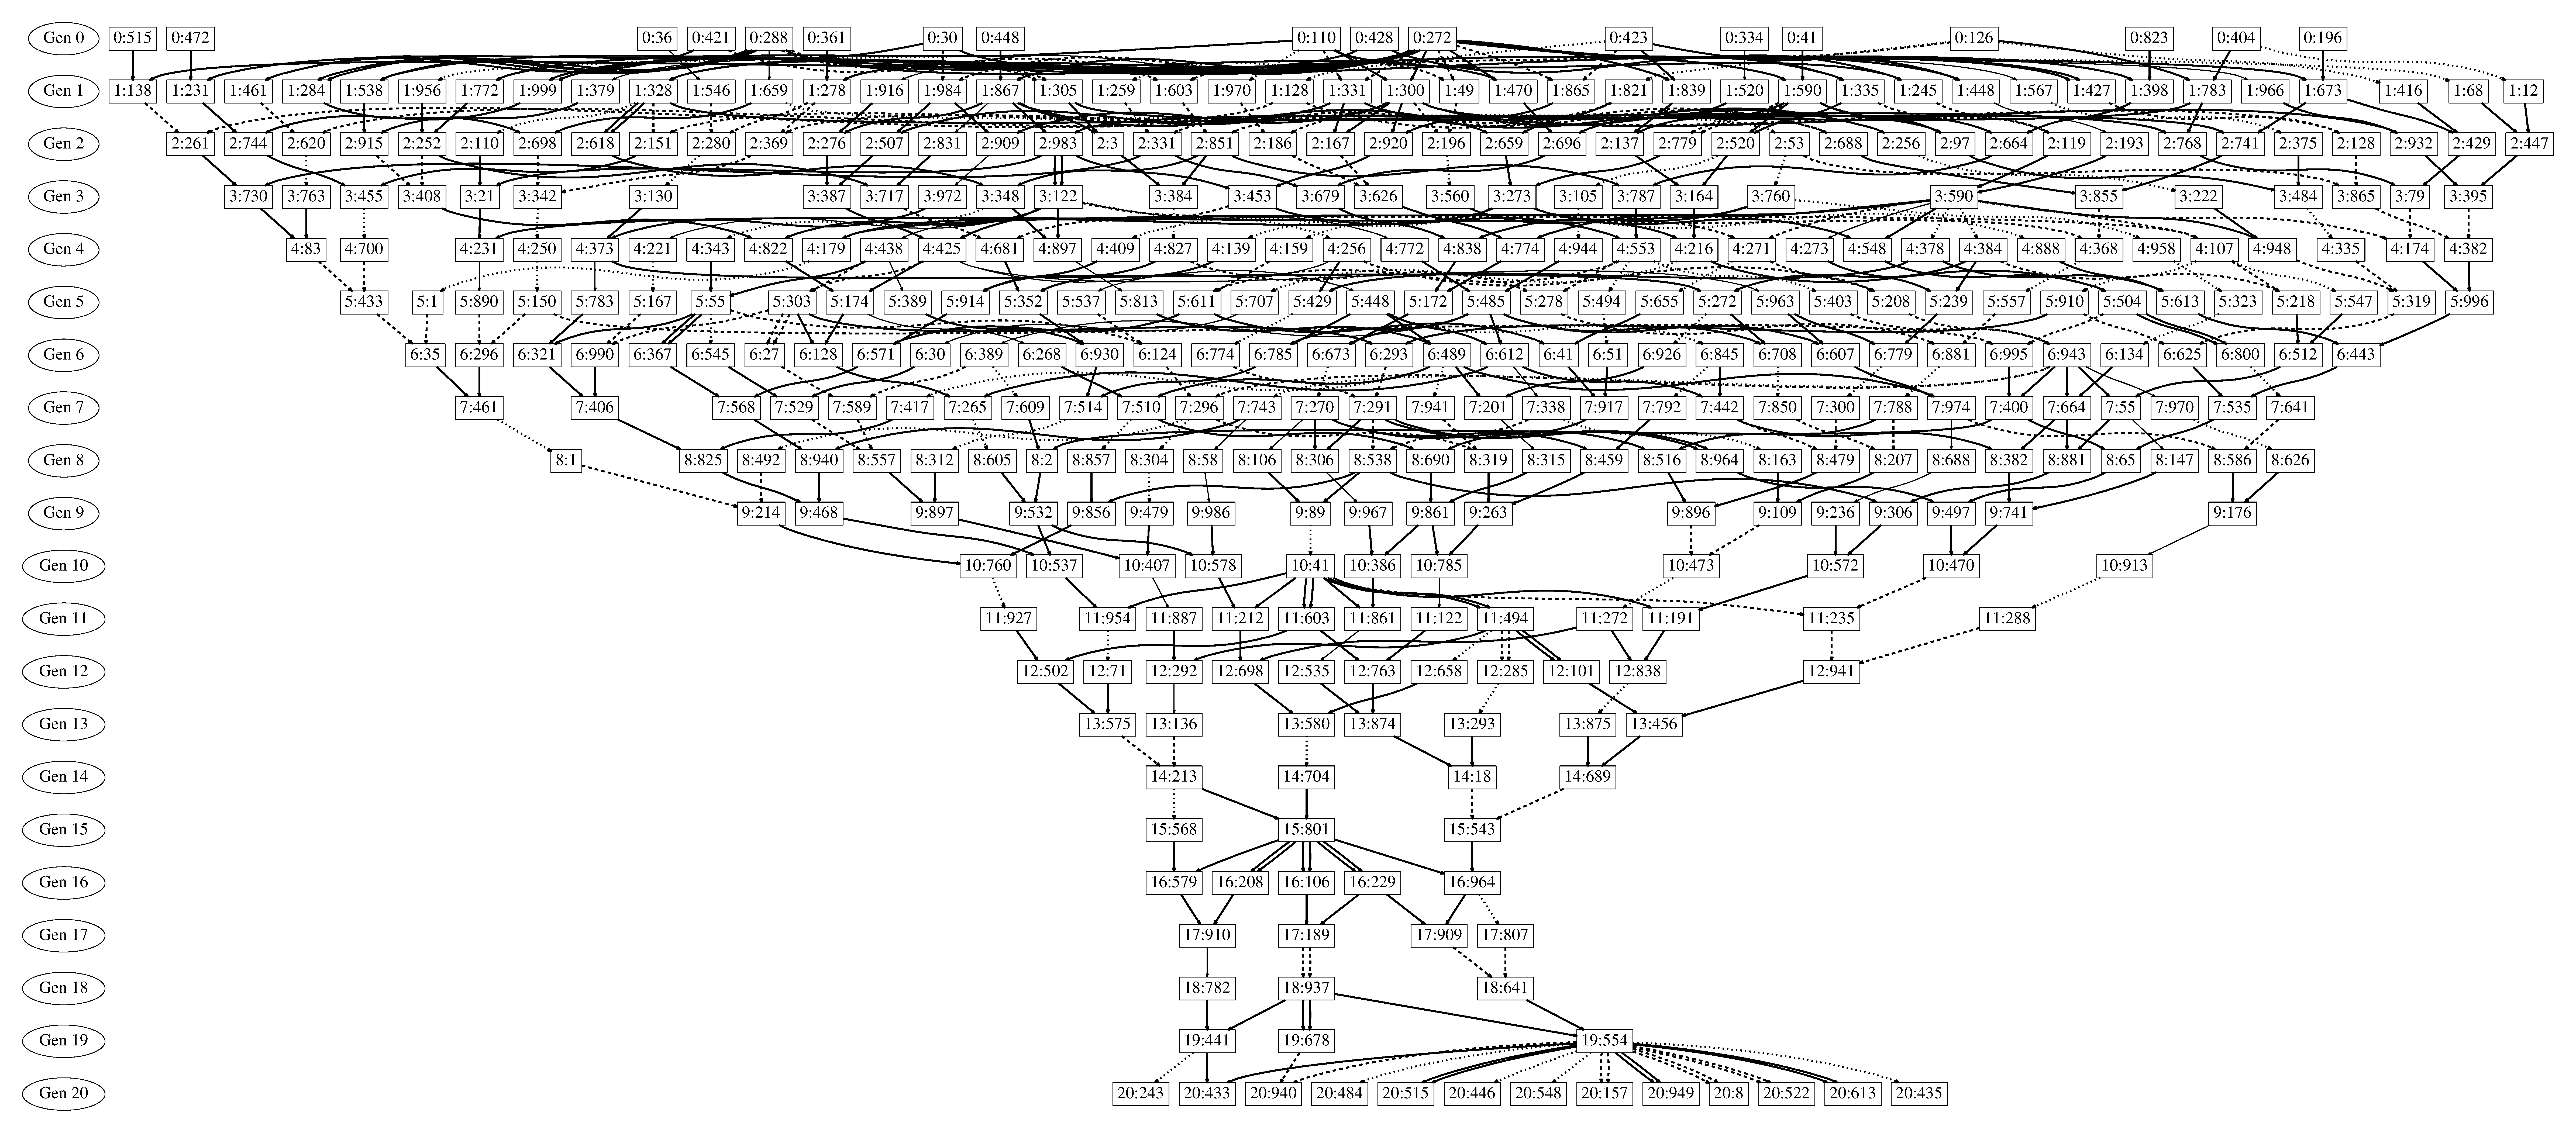
\includegraphics[width=\columnwidth]{../figures/run0_GPTP_2_font_30}
	\end{center}
	\caption{The full ancestry graph containing all the ancestors of the 13
		successful individuals. Individuals are represented with boxes, with the each generation being a row; the top row in the initial random
		population, and the bottom contains the 13 successful inidividuals.
		Edges represent parent-child relationships; see the text for 
		descriptions of the meaning of the particular edge decorations.}
	\label{fig:run0Labelled}       % Give a unique label
\end{sidewaysfigure}

The edges indicate the particular genetic operator (see Section~\ref{sec:background}) used to construct a child:
\begin{itemize}
	\item Dashed: alternation
	\item Dotted: uniform mutation
	\item Thin black lines: uniform close mutation
	\item Thick black lines: alternation followed by uniform mutation
\end{itemize}

This graph includes \emph{every} individual in this run that was an 
ancestor of one of the winners, i.e., every individual that could possibly have 
contributed genetic material to one of the winners. Note, however, that not
all these individuals actually contributed any genetic material to those
solutions. There are, for example, cases where one of the parents actually
contributed no material in a recombination (alternation) event, and cases where
a parent did contribute some genetic material, but that material was later
removed or replaced in subsequent mutations or recombinations. 

Conversely, while the individuals not represented in this graph are
guaranteed to have not contributed to the genetics of the successful
individuals, they might have still had some substantial impact on the
run's overall dynamics. The presence of those individuals and their
error vectors could certainly affect lexicase selection's choice of parents,
for example, which could substantially impact the dynamics.

\subsection{Genetic ancestry graph}

Despite the short length of this run, and the restriction to just displaying
ancestors of successful individuals, Figure~\ref{fig:run0Labelled} still
contains 394 nodes and 629 edges, making it difficult to analyze in full.

There were 13 successful individuals
in this run, most of which had identical simplified
programs. To further simplify the graph and the analysis, we picked\footnote{This choice 
	was somewhat arbitrary, but most of the 13 successful programs 
	simplify down to the same 9 instruction program, so the analysis would have 
	been the same in most cases even if we'd worked back from a different 
	successful individual.} 
one of the
successful individuals, namely 20:435, which was constructed via a single
instruction mutation from individual 19:554.
Individual 20:435's genome contained 194 genes, and its program had zero error on both
the training and testing cases.
The simplified program for 20:435 (which also passes all the tests)
contains only 9 instructions:
\begin{verbatim}
(\space \newline in1 string_replacechar print_string
in1 \space string_removechar string_length)
\end{verbatim}
This simplified program is actually quite readable, and has a similar
structure to what me might expect from a human solution.
The first five 
instructions (together on the first line) replace all the spaces in the input string 
with newlines (using the \texttt{string\_replacechar} instruction) and print the 
resulting string, thereby solving half the problem. 
The next four instructions (on the second line) remove all the spaces from
a fresh copy of the input string, compute the length and leave that on the
\texttt{:integer} stack as the ``returned'' result.

\begin{figure}[tb!p] %[b] sets the image at the bottom of the page; t = top, b = bottom, h = here%
	% \sidecaption
	% Use the relevant command for your figure-insertion program
	% to insert the figure file.
	% For example, with the graphicx style use
	\begin{center}
		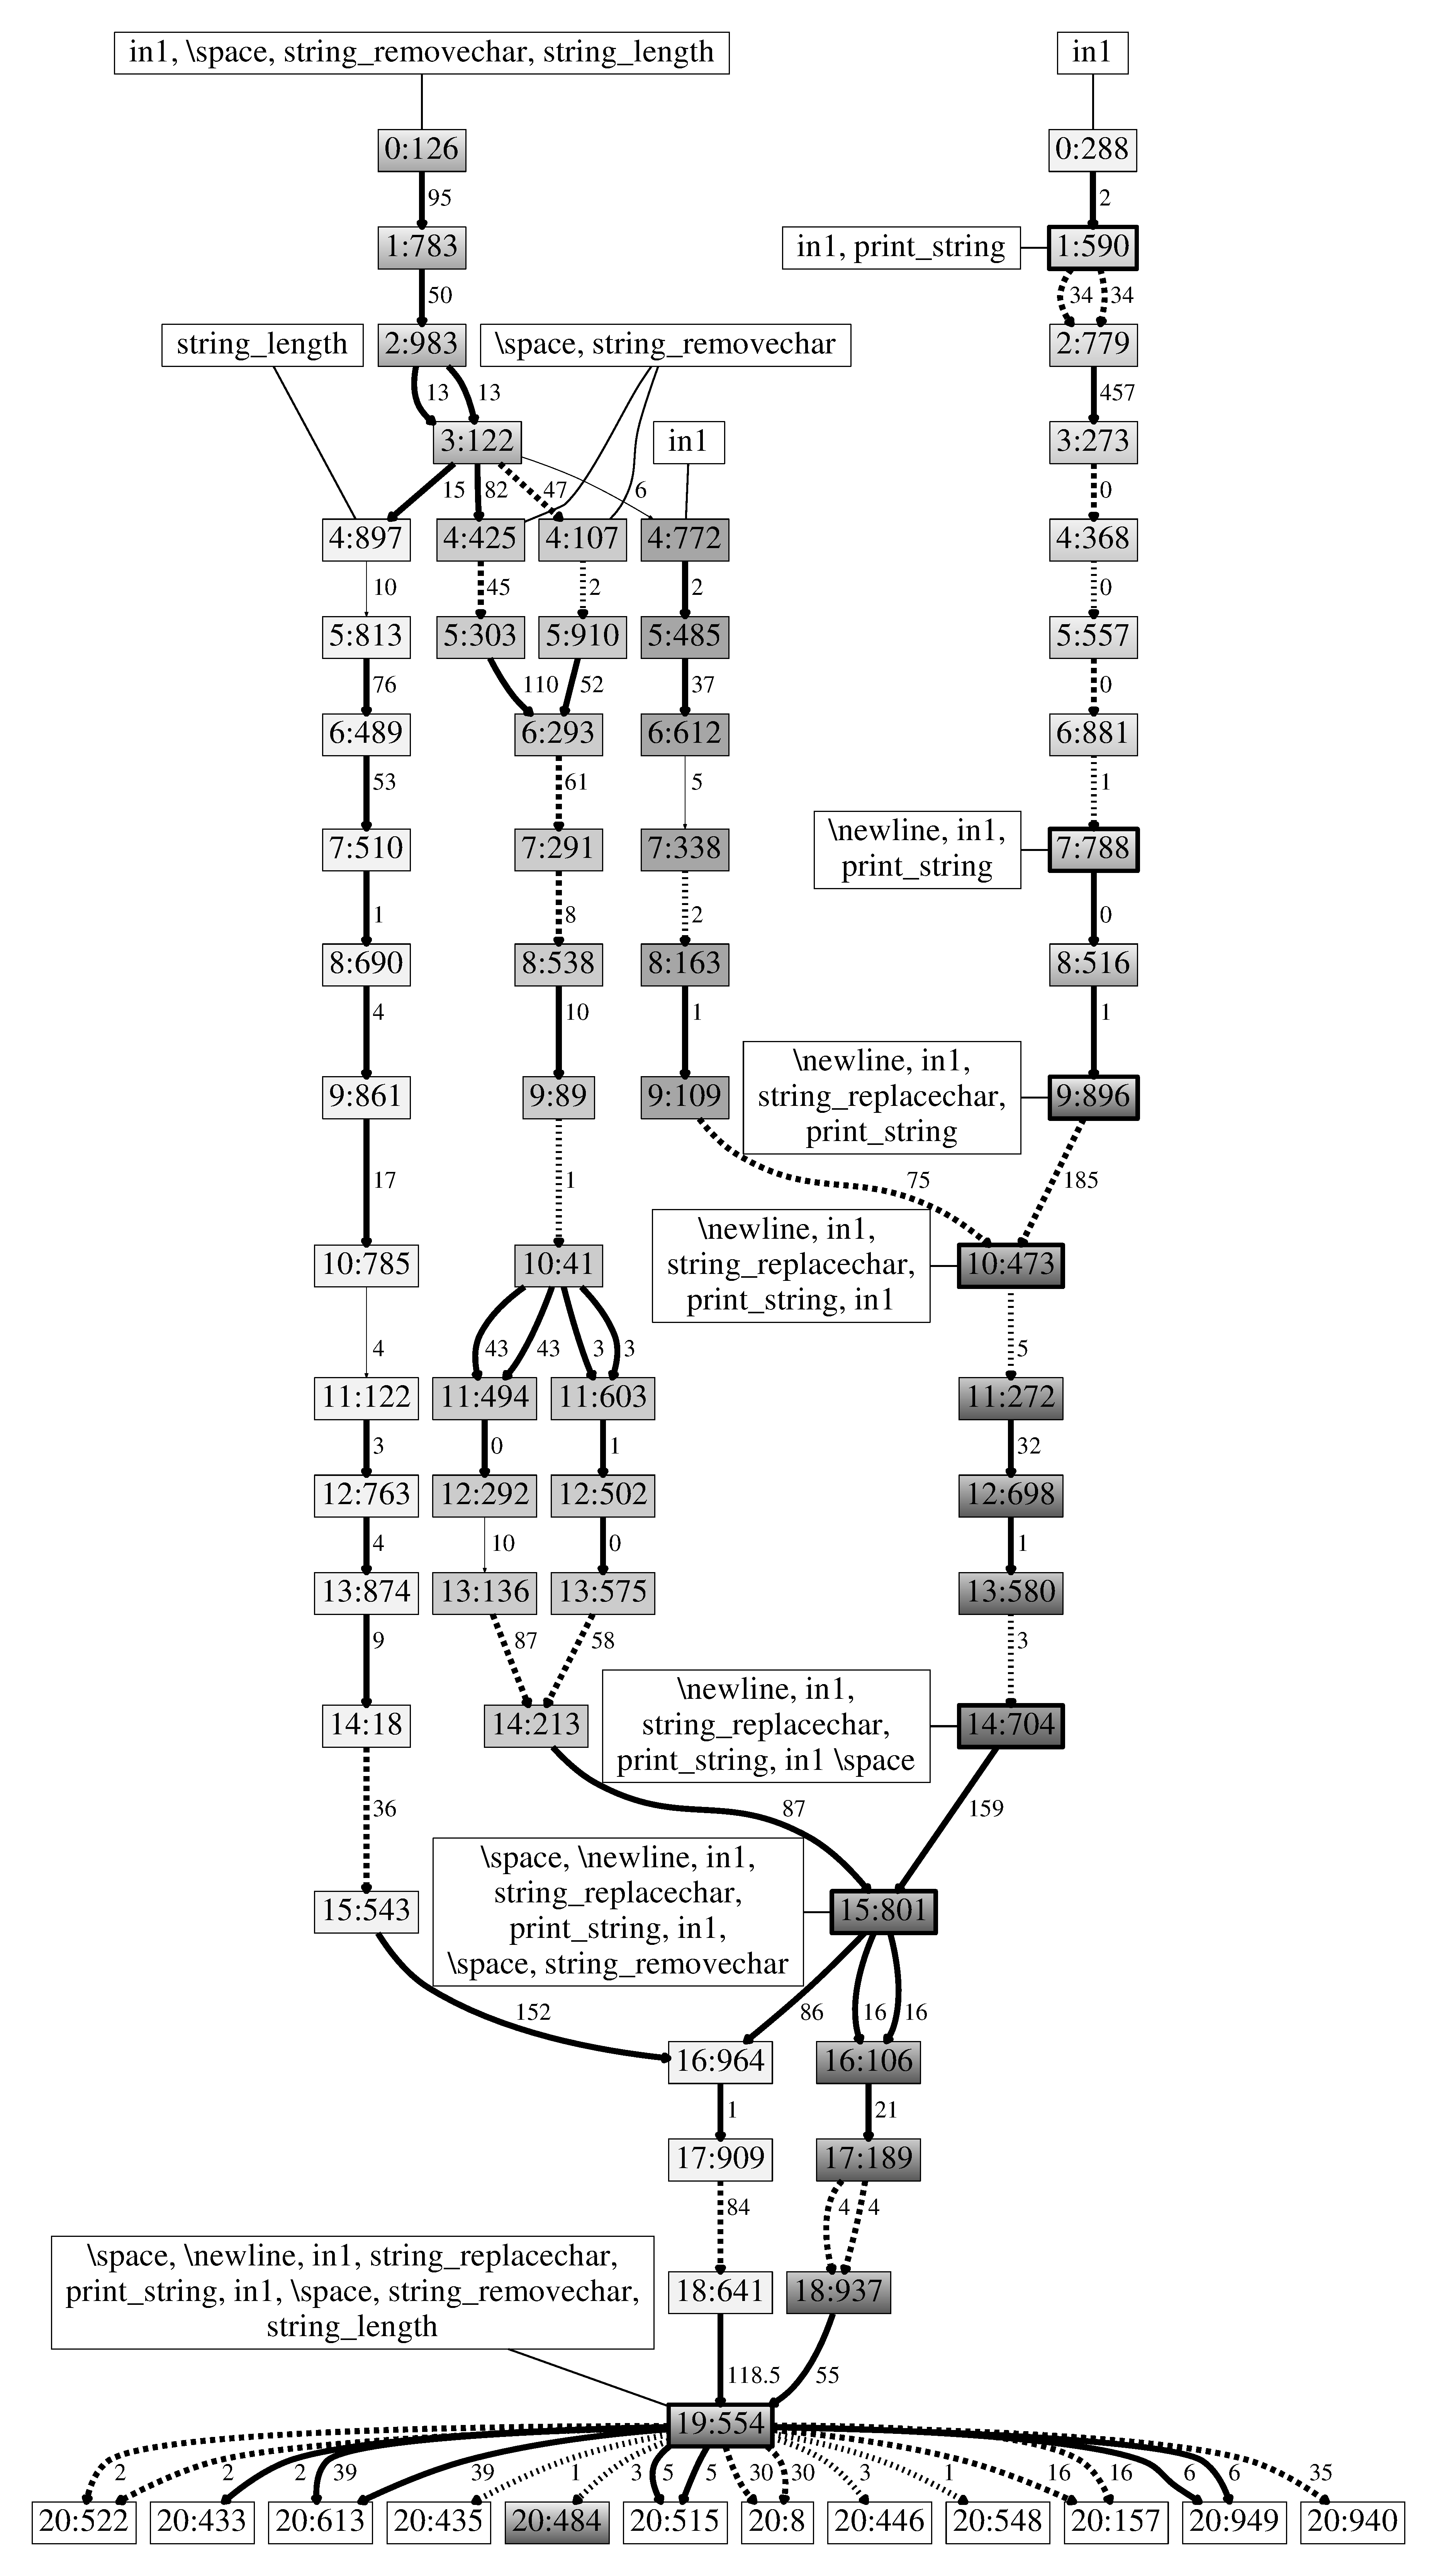
\includegraphics[height=0.95 \textheight]{../figures/filtered_fill}
	\end{center}
	\caption{The genetic ancestry version of the run's full ancestry graph.}
	\label{fig:run0Filtered}       % Give a unique label
\end{figure}

To simplify the graph in Figure~\ref{fig:run0Labelled}, we extracted the
subgraph containing only those individuals that contributed at least one
of these nine \emph{key instructions} to individual 20:435; see
Figure~\ref{fig:run0Filtered}.
Starting from 20:435 we traced backwards through it's 
ancestors, tracking where
the 9 key instructions came from. In doing so we found all of the members
in the full ancestry graph that contributed these important instructions. and then extracted the genetic
ancestry subgraph containing only these individuals. By cutting down on the 
number of individuals displayed
we have a much more readable and focused visualization of this important 
ancestry information.

The genetic ancestry graph in Figure~\ref{fig:run0Filtered} uses the same basic display of node and edge information
as the full ancestry graph.
However there are several additions that indicate how the 9 key instructions
flowed through the ancestry. 
First, we decorated nodes with boxes showing which of the 9 key instructions that were present in that individual. In most cases undecorated nodes
contain the same instructions as the most recent labeled ancestor; the
exceptions to this are individuals 16:964, 17:909, and 18:641, each of which 
contribute just the \texttt{string\_length} instruction inherited from 15:543. 
Next we added a thicker border to 
certain nodes, to indicate the introduction or combination of a key 
instructions via either mutation or crossover. Individual 1:590 is highlighted,
for example, because the key \texttt{print\_string} instruction was introduced 
their via uniform mutation, and individual 10:473 is highlighted because the
alternation of 9:109 and 9:896 brought together an \texttt{in1} instruction
from 9:109 (inherited from 0:126 via 4:772) with the four printing instructions 
from 9:896. Lastly
we used a grayscale color gradient to indicate which and how many of the 
instructions were present in an individual. The earlier of the 9 key 
instructions are assigned lighter colors in the gradient, and the later 
instructions are assigned darker gradient colors. So individuals like 7:338 
have a fairly ``flat'' gray because they contributed just a single
instruction from near the middle of the program, where 19:554 has a strong
gradiant because it contributed all 9 of the instructions.

The other important extension to the graph in Figure~\ref{fig:run0Filtered} 
is that we decorated each edge with the Damerau-Levenshtein distance (DL-distance)
between the genome vectors for each parent-child pair. The genome
vectors were generated by extracting the \texttt{:instruction}
\footnote{Instructions were treated as atomic symbols when computing the
	Damerau-Levenshtein distances; swapping a \texttt{exec\_if} with a \texttt{print\_string} would only add a
	distance of 1.}
and 
\texttt{:close} fields from each gene, and concatenating those into a
single sequence. So, for example, the genome of successful individual
20:435 starts

%\todo{Should this prefix of the genome be in a figure so it doesn't get broken up by things like page breaks?}
\begin{verbatim}
{:instruction boolean_and, :close 0} 
{:instruction boolean_shove, :close 0} 
{:instruction exec_do*count, :close 0} 
{:instruction exec_swap, :close 0} 
{:instruction integer_empty, :close 0}
...
\end{verbatim}

making the associated genome vector

\begin{verbatim}
boolean_and 0 boolean_shove 0 exec_do*count 0 
exec_swap 0 integer_empty 0 ...
\end{verbatim}

The Damerau-Levenshtein distance provides a succinct way to see when an individual has received a
large amount of genetic material from its parents. It also allows us to easily identify alternation
events that have mutation-like behavior, where there is only a small difference 
between to genome of one of the parents and the child.

\section{The (successful) end and how we got there}
\label{sec:successfulEnd}

As discussed earlier, individual 20:435's program simplfies down to just
nine instructions:
\begin{verbatim}
(\space \newline in1 string_replacechar print_string
in1 \space string_removechar string_length)
\end{verbatim}
where the first five instructions (the first line) handle the printing part
of the Replace Space With Newline problems, and the next four instructions
(the second line) handle the the requirement that the program returns the
number of non-space characters.

In this section we trace the origin of each of these nine instructions,
going back to their introduction either via a mutation or as an element 
of one of the initial, random programs in the first generation. It's clear
that each of these was ``necessary'' for the construction of this particular
solution, so knowing where they all came from and how they came together
should give us a valuable sense of the dynamics of this run. 
It's important to realize, however, that this will
never be the whole story. Push instructions and values can play an 
important role in subtle ways, e.g., as spacers on stacks that when
``counting'' is implemented with a stack depth command. Removal of
instructions can also be important. One key step in this run, for example, 
is the removal in the construction of 15:801 of an extraneous \texttt{print\_newline} present in 14:704; the presence of this
instruction caused the printed output to always have an error of one,
and its removal changed all of the 100 ``printing'' errors
from 1 to 0. All that said, however, we need some way to limit the number
of individuals and events to analyze, so here will focus on the how those
nine instructions trace through the ancestry.

It's also important to note that we didn't actually collect enough information
to always say for \emph{certain} where an instruction came from in a 
recombination event. There are numerous copies of instructions like
\texttt{in1} in most of the genomes, for example, and in principle any of them
in a parent could be the source of an \texttt{in1} in a child. In practice,
however, there are constrains of location and order that typically allowed
us to identify a single, unique source. There were a few places, however, where
judgement calls were made. In future work we're going to explore attaching
unique IDs to each gene and track not just parent-child relationships, but
also source-destination relationships among genes, as this will give us
certainty about the sources of genes, and allow us to automate more of the
analysis, all at the expense of larger databases.

Returning to the specific program,
it turns
out that the evolution of the first five instructions, those handling the
printing part of Replace Space With Newline, is largely independent of
the evolution of the last four instructions, which handle the return part
of the problem. The first five instructions, for example, all appear early 
in the genome for 20:435, between gene 9 and gene 24, while the last four 
all appear much later in the genome, between gene 107 and 175. As a consequence
we'll trace these two groups one at a time, then discuss the ``end game'' after
those two groups of instructions are brought together in individual 19:554.

\subsection{Printing: The first five instructions}
\label{sec:Printing}

The ancestry of the 5 instructions that solve the printing test
cases is fairly straightforward, and involves far more mutation than we
expected. Unlike the return case instructions described below 
(Section~\ref{sec:Returning}), here there is a clear linear path for these 
instructions. They are introduced over time, and they 
are never split apart into branches to be recombined later.

Starting at the top-right of Figure~\ref{fig:run0Filtered} with individual 0:288, only
one of the key instructions, \texttt{in1}, was present in that individual from 
the initial randomly generated population. The other 4 of the 5 key printing 
instructions were introduced over time
through a series of uniform mutations. The second of these 5 key instructions was introduced in individual 1:590 via a point
mutation converting a piece of 0:288's genome into a \texttt{print\_string} instruction. These two
instructions are passed along this branch until they are joined by the next important instruction,
\texttt{\textbackslash newline}, introduced in 7:788 again via uniform
mutation.
After descending another 2 generations these three instructions were joined by \texttt{string\_replacechar}
in 9:896 via yet another uniform mutation. 
The final of these 5 key instructions, \texttt{\textbackslash space} was
added in generation 14 via a uniform mutation of 13:580 into 14:704, thus completing the five key printing
instructions. These five instructions were then passed down as a group through 15:801 to the winners.

The impact of these instruction additions can be seen in the individuals'
error vectors, as each addition
was accompanied by a shift in the printing test cases. Sometimes the effect was 
minimal, with both small positive and small negative changes
in the errors for different test cases, while other times the change led to 
dramatic improvements. As an example of a dramatic improvement, when
\texttt{print\_string} was introduced into 1:590, for example, the error on 
nearly all of the 100 printing test improved, with only a few showing an 
increased error; the total error for 1:590 across all 200 test cases was 
492, where it's parents (0:41\footnote{Individual 0:41 isn't shown in 
	Figure~\ref{fig:run0Filtered} since it didn't contribute any of the 9 key 
	instructions to 1:590 or, ultimately, 20:435.} and 0:288) has total errors 
of 1,594 and 1,154 respectively.
Later, in the creation of 14:704 via mutation from 13:580 all of the 
printing test scores became 1. This was in general an \emph{vital} step, 
but did lead to an increased error on a few tests that had passed with no 
error in 13:580; the total error of 14:704 was 922, where the 
total error of 13:580 was a slightly worse 1,125.

\subsection{Returning: The last four instructions}
\label{sec:Returning}

The last four ``returning'' instructions were present in the right order and in 
rough proximity in the very first generation, in individual 0:126. The first of these instructions (\texttt{in1}) was on gene 75 of the genome, the next two
(\texttt{\textbackslash space} and \texttt{string\_removechar}) were on 
genes 89 and 94, and then the final instruction (\texttt{string\_length}) 
was on line 141 (out of a total of 161 genes in that initial genome).

Despite the fact that this individual had ``all the right stuff'', it's error
vector had very few zeros, i.e., it was rarely correct, highlighting
the fact that the presence or absence of other instructions can profoundly
impact a program's behavior. 0:126 was, however, quite good for a randomly
generated program, with all it's errors being under 20, and most being in
the single digits. It was selected 45 times to be a parent, making it the
seventh most selected parent in the initial generation, and one of only 48
individuals in the initial generation that received any selections. 
(The most selected
parent in that generation, 0:272, was selected 762 times, but ultimately
contributed no genes to the winning individual and therefore is not shown in the graph.)

Those four instructions were passed on as a group, with nearly the same 
relative positions in the genomes, from 0:126 through 1:783 and 2:983 
to 3:122 (see Figure~\ref{fig:run0Filtered}). 
3:122 was the third most selected individual in its generation
and had 100 children, several of which went on to carry one or more of
these four instructions forward to individual 19:554 when they were finally
reunited in the positions that would ultimately lead to success. In particular
there were three distinct branches coming from 3:122, each of which will
be discussed below.

\subsubsection{Branch 4:772 and the carriers of \texttt{in1}}
\label{sec:4:772}

Individual 4:772 inherited the copy of the first instruction,
\texttt{in1}, that would ultimately form part of the solution. This was
transmitted down to 9:109 where it was recombined with 
9:896 which, as mentioned above in Section~\ref{sec:Printing}, carried
all but one of the first five ``printing'' instructions. 

This recombination
led to individual 10:473, which then had 4 of the 5 ``printing'' instructions,
as well as the \texttt{in1} that would be the first of the 4 ``returning''
instructions. These five instructions were then passed down to 14:704, 
along with the 
\texttt{\textbackslash space} introduced by mutation in 14:704. 14:704 was
one of the parents of 15:801, a recombination which will be described in the
discussion of the next branch.

\subsubsection{Branches 4:425, 4:107, and multiple blocks}
\label{sec:4:425}

3:122 contained a block of 25 genes % genes 77 to 101
that contain the two middle instructions in the ``returning''
code, \texttt{\textbackslash space} and \texttt{string\_removechar}.
This block was replicated in both 4:425 and 4:107, and then passed,
respectively, to 5:303 and 5:910. 5:303 and 5:910 then recombined
to create 6:293, which ended up having two complete copies of this
block of genes. % genes 67 to 91 and 100 to 124.

These two copies of this block were then copied from 7:291 down through 10:41,
to both 13:136 and 13:575. When these recombined to form 14:213
we ended up with \emph{three} near copies of the block. These blocks
were no longer identical due to small changes caused by earlier
genetic operations, but each block still contained over 20 genes shared,
including the two key instructions,
\texttt{\textbackslash space} and \texttt{string\_removechar},
still four instructions apart.

All three of these blocks (and their three copies of these two ``final''
instructions) were passed on to 15:801 in the recombination of 14:213 and
14:704. 14:704 also bequeathed to 15:801 all of its six ``final'' 
instructions, meaning that 15:801 had all but one of those 9
instructions, missing only the final \texttt{string\_length}.

\subsubsection{Branch 4:897 and the carriers of \texttt{string\_length}}
\label{sec:4:897}

4:897 and its descendants carried the copy of the last instruction, 
\texttt{string\_length}, that would ultimately form part of the solution. 
This was transmitted all the way down to
18:641 without any significant interactions with other ``final instructions'',
as is reflected in the almost entirely linear ancestry from 4:897 to 18:641 
in Figure~\ref{fig:run0Filtered}.

There was one potentially interesting interaction with the other branches, 
when 15:543 combined with 15:801 to create 16:964. In this recombination event,
however, 15:801 did not contribute any of the 9 key instructions to 16:964. 
15:543, on the other hand, transmitted the crucial missing 
\texttt{string\_length} gene that had been passed down since our starting 
random generation, and which went on to be part of the solution in 20:435.

\subsection{From 19:554 to the end, and the final adjustments}

19:554 was the result of a recombination of 18:641 and 18:937, which finally
brought together all nine of the ``final'' instructions. 18:937 contributed
the first 8 instructions, and 18:641 contributed the final 
\texttt{string\_length} instruction. Individual 19:554 didn't \emph{quite} solve the
problem, however, it did have three ``return'' test cases with error 1. These three test cases turned out to be the only cases with an input of a single character.

These errors were fairly easy to rectify, however, as evidenced by the 
fact that 12 of 19:554's 747 offspring (or 1.6\%) were indeed successful.
Two of these successful children (20:435 and 20:548) were the result of 
mutating a \emph{single} instruction. The key change brought about by the 
mutation that led to 20:435 
caused an instance of the instruction \texttt{string\_butlast} to not operate. 
In 19:554 this \texttt{string\_butlast} was incorrectly removing the one and 
only character
from the input string when the input consisted of a single character string, so 
the suppression of that instruction led to a perfect solution.

\section{Discussion}
\label{sec:discussion}

The trace in Section~\ref{sec:successfulEnd} provides a sense of where all
the key instructions came from, and indicates several of the key moments in the
evolutionary process. In this section we'll provide some summary information
as well as highlighting both some general patterns and a few important events.

Table~\ref{tab:operatorCounts} enumerates the number and proportions 
of individuals constructed via the four genetic operators, first across the
entire run (so all of the 20,000 individuals generated after the initial
random population), then for the ancestry graph in 
Figure~\ref{fig:run0Labelled} (394 total nodes, 
376 constructed after the initial generation), and finally for the genetic 
ancestry
graph in Figure~\ref{fig:run0Filtered} (62 total nodes, 60 constructed after 
the initial generation). The percentages in the ``Entire run'' column match
the settings in the run configuration, which specified using alternation 
followed by uniform mutation 50\% of the time, alternation alone 20\% of the 
time, uniform mutation 20\% of the time, and uniform close mutation the 
remaining 10\% of the time. 
The other two columns have similar percentages,
suggesting that there wasn't a large skew away from those parameter values,
and that none of the genetic operators were particularly over- or 
under-represented in the ancestry graphs.

\begin{table}[t]
	\begin{tabular}{lrrr}
		\textbf{Genetic operator} & \textbf{Entire run} & $\;$ \textbf{Full ancestry graph} & $\;$ \textbf{Genetic ancestry graph} \\ 
		\hline
		Alternation + uniform mutation & 9,985 (50\%) & 186 (49\%) & 39 (54\%) \\ 
		Alternation & 4,001 (20\%) & 67 (18\%) & 17 (24\%) \\ 
		Uniform mutation & 4,026 (20\%) & 83 (22\%) & 11 (15\%) \\ 
		Uniform close mutation & 1,988 (10\%) & 40 (11\%) & 5 (7\%)
	\end{tabular} 
	\caption{The numbers and proportions of individuals constructed using
		the different genetic operators. Total percentages might not equal 100\% due to rounding.}
	\label{tab:operatorCounts}
\end{table}

While there are numerous alternations in the genetic ancestry graph, it's worth
noting that many of the DL-distances (the edge labels in 
Figure~\ref{fig:run0Filtered}) are fairly small, even when alternation was
involved, as can be seen in Figure~\ref{fig:alt:DLdist:distribution}. Of the
53 alternations in the genetic ancestry graph
(ignoring those leading to a successful individual in 
generation 20), 21 had DL-distances of 10 or less, 6 had DL-distances of just 1,
and 5 had DL-distances of 0 (the child was an exact copy of a parent).
One might assume that this is partly due to the six 
self-cross alternations, where the same individual served as both parents, 
such as individual 16:106 having 15:801 as both of its parents.\footnote{These self-crosses are likely a result of hyperselection events due to lexicase 
	selection~\cite{Helmuth:2016:GECCO}.} In fact, however, most of the 
self-crosses in the genetic ancestry graph had higher than median DL-distances.

\begin{figure}[t]
	\begin{center}
		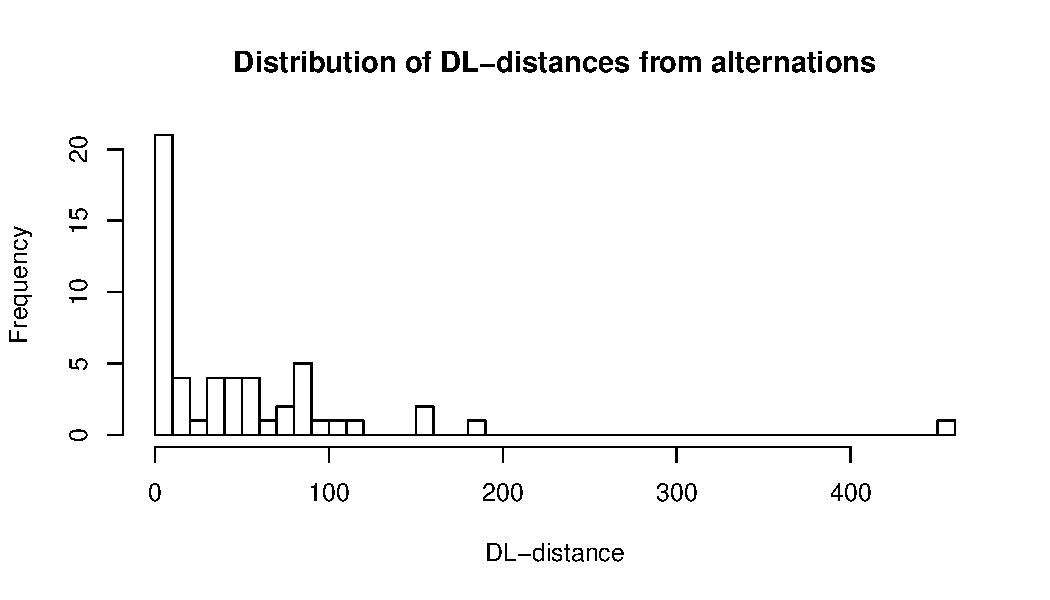
\includegraphics[width=0.9\textwidth]{../figures/Alternation_dl_distance_distribution}
	\end{center}
	\vspace{-0.5 cm}
	\caption{The distribution of DL-distances for all the alternation events 
		in the genetic ancestry graph (Figure~\ref{fig:run0Filtered}) whether 
		or not they were followed by uniform mutation. This does not include
		the alternations leading to successful individuals in the final \
		generation since those were almost all self-crosses, which skew towards 
		smaller DL-distances.}
	\label{fig:alt:DLdist:distribution}
\end{figure}

These very small DL-distances mean that many of the alternations were 
effectively acting as mutation-like events. The steps from individual
15:801 to 18:937, for example, are all alternations (possibly followed
by mutations), but in fact almost every change in that sequence was due to
gene deletions or duplications in those alternation events. There were 3
mutated genes in that sequence of steps, along with 12 deleted genes and the
duplication of a block of 7 genes.

Since the genetic ancestry graph (and thus the data in 
Figure~\ref{fig:alt:DLdist:distribution}) only includes individuals that 
actually
contributed one of the nine key instructions, in many cases the second parent
in alternation events isn't included; these DL-distances are in general
higher than those listed. This isn't surprising, as a parent with a small
DL-distance is very similar to the child, and thus likely to have contributed
most of the important genetic material. There are, however, a few exceptions 
to this pattern. Perhaps the most extreme is in the creation of individual
3:273 via alternation between 2:659 and 2:779. Individual 2:659 is not included
in the genetic ancestry graph in Figure~\ref{fig:run0Filtered} because it didn't
contribute any of the nine key instructions to 3:273, whereas 2:779 contributed
two such instructions. However the DL-distance between 3:273 and 2:779 was 457, 
which was much greater than the distance to 2:659, which was only 50. So despite
being much more similar to 2:659 and getting most of its genetic material from
that parent, the material that ultimately contributed to the solution all came
from the other parent (2:779).

Not all alternation events in Figure~\ref{fig:run0Filtered} could effectively be seen as
mutation events, however. The construction of 15:801, for example,
was in many ways what we imagine when we think about
crossover events, combining significant genetic material and significant functionality from two different parents. It was also a key point in the run,
as 15:801 was the first individual to be correct on all of the ``printing''
test cases, and it was also correct on 26 of the 100 ``returning'' test cases.

Individual 15:801 was created through the recombination of 14:704 and 14:213,
via alternation followed by uniform mutation. 
Table~\ref{tab:15:801} shows the simplified programs of 
both parents and the child,
aligned to indicate where the various instructions likely came from. The key
observation is that 15:801 received most of its initial genetic material from 
14:704 (most of genes 1-6), followed by a large section (genes 7-35) taken
almost entirely from 14:213's genome. Interestingly, the transition between 14:704 and 15:801 involved a simple but crucial change that fixed all the
printing cases. 14:704 had an error of exactly 1 on all the printing cases
due to an extra \texttt{print\_newline} (line 37 in Table~\ref{tab:15:801}).
In the recombination this gene wasn't passed on to 15:801, which led to a
perfect score of 0 on all those test cases. The performance of 15:801 on
the return test cases wasn't quite as strong as that of its other parent,
14:213, but was generally better than 14:704's performance on those test cases. 15:801 went on to receive a large number of selections (595) and being
a parent of just over half the next generation (501 individuals).

\begin{table}
	\begin{tabular}{l|rl|l}
		\textbf{14:704} & & \textbf{15:801} & \textbf{14:213} \\
		\hline
		& 0 & & \texttt{(in1} \\ 
		\texttt{(\textbackslash space} & 1 & \texttt{(\textbackslash space} & \\ 
		\texttt{ \textbackslash newline} & 2 & \texttt{ \textbackslash newline} &  \\ 
		& 3 & \texttt{ exec\_dup} &  \\ 
		\texttt{ in1} & 4 & \texttt{ in1} &  \\ 
		\texttt{ string\_replacechar} & 5 & \texttt{ string\_replacechar} &  \\ 
		\texttt{ print\_string} & 6 & \texttt{ print\_string} & \texttt{ print\_string} \\ 
		& 7 & \texttt{ exec\_dup} & \texttt{ exec\_dup} \\ 
		& 8 &  & \texttt{ exec\_s} \\ 
		& 9 &  & \texttt{ (exec\_dup} \\ 
		& 10 &  & \texttt{ \ (exec\_rot} \\ 
		& 11 & \texttt{ (string\_eq} & \texttt{ \ \ (string\_eq} \\
		& 12 & &  \texttt{ \ \ \ string\_fromboolean)} \\ 
		& 13 &  & \texttt{ \ \ char\_eq} \\ 
		& 14 & & \texttt{ \ \ (string\_emptystring} \\
		& 15 & &  \texttt{ \ \ \ boolean\_stackdepth} \\
		& 16 & & \texttt{ \ \ \ in1} \\
		& 17 & & \texttt{ \ \ \ integer\_gt)} \\ 
		& 18 &  & \texttt{ \ \ string\_emptystring} \\ 
		& 19 & \texttt{ \ \textbackslash space} & \texttt{ \ \ \textbackslash space} \\ 
		& 20 & \texttt{ \ string\_dup} & \texttt{ \ \ string\_dup} \\ 
		& 21 & \texttt{ \ string\_removechar} & \texttt{ \ \ string\_removechar} \\
		& 22 & \texttt{ \ string\_rot} & \\
		& 23 & & \texttt{ \ \ boolean\_pop} \\ 
		& 24 &   & \texttt{ \ \ in1} \\ 
		& 25 &   & \texttt{ \ \ string\_butlast} \\ 
		& 26 &   & \texttt{ \ \ string\_last} \\ 
		& 27 &   & \texttt{ \ \ string\_parse\_to\_chars} \\
		& 28 &   & \texttt{ \ \ exec\_when} \\ 
		& 29 &   & \texttt{ \ \ string\_dup} \\
		& 30 &   & \texttt{ \ \ string\_removechar} \\
		& 31 & \texttt{ \ string\_last} & \texttt{ \ \ string\_last} \\
		& 32 & \texttt{ \ string\_parse\_to\_chars} & \texttt{ \ \ string\_parse\_to\_chars} \\
		& 33 & \texttt{ \ string\_rot)} & \texttt{ \ \ string\_rot)} \\
		& 34 & \texttt{ in1} & \texttt{ \ in1)} \\
		& 35 & \texttt{ string\_stackdepth)} & \texttt{ string\_stackdepth)} \\
		\texttt{ boolean\_stackdepth} & 36 & & \\
		\texttt{ print\_newline)} & 37 & & \\
	\end{tabular}
	\caption{The details of the recombination event (alternation followed by
		uniform mutation) that created individual
		15:801 (center) from parents 14:704 (left) and 14:213 (right) showing
		the \emph{simplified} programs for those individuals (see
		Section~\ref{sec:background}). This shows that individual 15:801 was
		essentially constructed from a short prefix of 14:704 and a longer suffix of 14:213.}
	\label{tab:15:801}
\end{table}

\section{Conclusions and future work}
\label{sec:conclusions}

Here we traced through the genetic ancestry of a short, successful genetic programming run. While the run was short, it used an ``industrial strength''
PushGP system on a
non-trivial problem that required the manipulation of strings and integers in multiple
ways, and a combination of both printing and returning results. We used graph
database tools to create
ancestry and genetic ancestry graphs, which we were then able to use to 
visualize and analyze this run. The resulting graphs
show the progression of the run and highlight important moments such as key
recombination events, gene deletions and duplications, and the introduction
of key instructions via mutation. By tracing through the genetic ancestry tree we were able to learn more about how both alternation and mutation played a role in finding a solution.

While we were able to do this for a small run, currently too much of the
process is manual for this to scale to larger runs or multiple sets of runs.
A key next step in further automating this kind of analysis is automating the 
process of comparing individuals, especially at the genome level. Tracing
each key instruction back through the ancestry graph can be complicated, in
part because there are often many different instances of the instruction being traced; individual 19:554, for example, had four instances of 
\texttt{\textbackslash space}, but only three of those were present in its
simplified program, and only two went on to be part of the simplified
successful program in 20:435. In this case we were able to deal with these
problems by using contextual clues such as order in the genome and surrounding
instructions, not unlike how biologists track gene sequences in organisms.
To make this process more automatic and exact, however, we'll need to save additional
information with the individual genes that allows us to know exactly where they 
came from.

It would also be valuable to improve our ability to understand and compare
program behaviors. We can easily compare genomes and error vectors,
and reasonably compare program \emph{texts}, comparing program \emph{behaviors}
is much less straightforward. While the simplified program for individual
20:435 is quite short and understandable, the unsimplified program contains
195 instructions, which include a number of complex looping constructs. These
are obviously not necessary for the semantics of the program, but they are
present in the code that is being tested, and the genes that create those
instructions are part of the genome that is being manipulated and inherited.
And while those instructions might be removable from 20:435 at the end 
of the run, it's likely that many of those instructions played some
meaningful role in an ancestor that contributed to that ancestor's selection.

Lastly the prevalence of numerous alternation events in the 
gene ancestry graph that turned out to be just gene deletions or duplications 
suggests that it might be valuable to include deletion and replication 
mutations as stand-alone operators, instead of requiring that such events
occur via lucky alternations.

\begin{acknowledgement}
	Emma Sax, Laverne Schrock, and Leonid Scott helped 
	with the initial computation and analyses of the differences between the 
	parents and children discussed here. William Tozier provided a host of 
	ideas and feedback all through the process, as did numerous members
	of the Hampshire College Computational Intelligence lab.
	
	We are very grateful to all the participants in the 2016 Genetic Programming Theory and Practice (GPTP) workshop for their enthusiasm, ideas, and support. In particular we'd like to thank William Tozier,
	Stephan Winkler, and Wolfgang Banzhaf for their feedback on an earlier
	draft. Finally, thanks to the GPTP organizers; without their hard work none of those other valuable conversations would have occurred.
	
	This material is based upon work supported by the National Science Foundation under Grants No. 1129139 and 1331283. Any opinions, findings, and conclusions or recommendations expressed in this publication are those of the authors and do not necessarily reflect the views of the National Science Foundation.
\end{acknowledgement}

\bibliographystyle{spmpsci}
\bibliography{gp-bibliography,mcphee}

%\section{Section Heading}
%\label{sec:1}
%Use the template \emph{chapter.tex} together with the Springer document class SVMono (monograph-type books) or SVMult (edited books) to style the various elements of your chapter content in the Springer layout.
%
%Instead of simply listing headings of different levels we recommend to
%let every heading be followed by at least a short passage of text.
%Further on please use the \LaTeX\ automatism for all your
%cross-references and citations. And please note that the first line of
%text that follows a heading is not indented, whereas the first lines of
%all subsequent paragraphs are.
%
%\section{Section Heading}
%\label{sec:2}
%% Always give a unique label
%% and use \ref{<label>} for cross-references
%% and \cite{<label>} for bibliographic references
%% use \sectionmark{}
%% to alter or adjust the section heading in the running head
%Instead of simply listing headings of different levels we recommend to
%let every heading be followed by at least a short passage of text.
%Further on please use the \LaTeX\ automatism for all your
%cross-references and citations.
%
%Please note that the first line of text that follows a heading is not indented, whereas the first lines of all subsequent paragraphs are.
%
%Use the standard \verb|equation| environment to typeset your equations, e.g.
%%
%\begin{equation}
%a \times b = c\;,
%\end{equation}
%%
%however, for multiline equations we recommend to use the \verb|eqnarray| environment\footnote{In physics texts please activate the class option \texttt{vecphys} to depict your vectors in \textbf{\itshape boldface-italic} type - as is customary for a wide range of physical subjects}.
%\begin{eqnarray}
%a \times b = c \nonumber\\
%\vec{a} \cdot \vec{b}=\vec{c}
%\label{eq:01}
%\end{eqnarray}
%
%\subsection{Subsection Heading}
%\label{subsec:2}
%Instead of simply listing headings of different levels we recommend to
%let every heading be followed by at least a short passage of text.
%Further on please use the \LaTeX\ automatism for all your
%cross-references\index{cross-references} and citations\index{citations}
%as has already been described in Sect.~\ref{sec:2}.
%
%\begin{quotation}
%Please do not use quotation marks when quoting texts! Simply use the \verb|quotation| environment -- it will automatically render Springer's preferred layout.
%\end{quotation}
%
%
%\subsubsection{Subsubsection Heading}
%Instead of simply listing headings of different levels we recommend to
%let every heading be followed by at least a short passage of text.
%Further on please use the \LaTeX\ automatism for all your
%cross-references and citations as has already been described in
%Sect.~\ref{subsec:2}, see also Fig.~\ref{fig:1}\footnote{If you copy
%text passages, figures, or tables from other works, you must obtain
%\textit{permission} from the copyright holder (usually the original
%publisher). Please enclose the signed permission with the manuscript. The
%sources\index{permission to print} must be acknowledged either in the
%captions, as footnotes or in a separate section of the book.}
%
%Please note that the first line of text that follows a heading is not indented, whereas the first lines of all subsequent paragraphs are.
%
%% For figures use
%%
%\begin{figure}[b]
%\sidecaption
%% Use the relevant command for your figure-insertion program
%% to insert the figure file.
%% For example, with the graphicx style use
%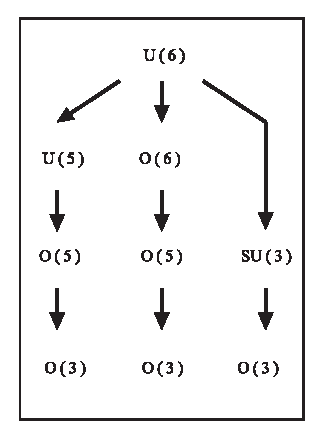
\includegraphics[scale=.65]{figure}
%%
%% If no graphics program available, insert a blank space i.e. use
%%\picplace{5cm}{2cm} % Give the correct figure height and width in cm
%%
%\caption{If the width of the figure is less than 7.8 cm use the \texttt{sidecapion} command to flush the caption on the left side of the page. If the figure is positioned at the top of the page, align the sidecaption with the top of the figure -- to achieve this you simply need to use the optional argument \texttt{[t]} with the \texttt{sidecaption} command}
%\label{fig:1}       % Give a unique label
%\end{figure}
%
%
%\paragraph{Paragraph Heading} %
%Instead of simply listing headings of different levels we recommend to
%let every heading be followed by at least a short passage of text.
%Further on please use the \LaTeX\ automatism for all your
%cross-references and citations as has already been described in
%Sect.~\ref{sec:2}.
%
%Please note that the first line of text that follows a heading is not indented, whereas the first lines of all subsequent paragraphs are.
%
%For typesetting numbered lists we recommend to use the \verb|enumerate| environment -- it will automatically render Springer's preferred layout.
%
%\begin{enumerate}
%\item{Livelihood and survival mobility are oftentimes coutcomes of uneven socioeconomic development.}
%\begin{enumerate}
%\item{Livelihood and survival mobility are oftentimes coutcomes of uneven socioeconomic development.}
%\item{Livelihood and survival mobility are oftentimes coutcomes of uneven socioeconomic development.}
%\end{enumerate}
%\item{Livelihood and survival mobility are oftentimes coutcomes of uneven socioeconomic development.}
%\end{enumerate}
%
%
%\subparagraph{Subparagraph Heading} In order to avoid simply listing headings of different levels we recommend to let every heading be followed by at least a short passage of text. Use the \LaTeX\ automatism for all your cross-references and citations as has already been described in Sect.~\ref{sec:2}, see also Fig.~\ref{fig:2}.
%
%For unnumbered list we recommend to use the \verb|itemize| environment -- it will automatically render Springer's preferred layout.
%
%\begin{itemize}
%\item{Livelihood and survival mobility are oftentimes coutcomes of uneven socioeconomic development, cf. Table~\ref{tab:1}.}
%\begin{itemize}
%\item{Livelihood and survival mobility are oftentimes coutcomes of uneven socioeconomic development.}
%\item{Livelihood and survival mobility are oftentimes coutcomes of uneven socioeconomic development.}
%\end{itemize}
%\item{Livelihood and survival mobility are oftentimes coutcomes of uneven socioeconomic development.}
%\end{itemize}
%
%\begin{figure}[t]
%\sidecaption[t]
%% Use the relevant command for your figure-insertion program
%% to insert the figure file.
%% For example, with the option graphics use
%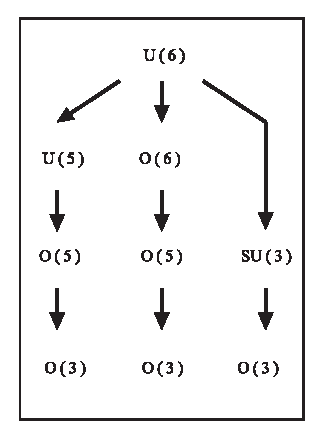
\includegraphics[scale=.65]{figure}
%%
%% If no graphics program available, insert a blank space i.e. use
%%\picplace{5cm}{2cm} % Give the correct figure height and width in cm
%%
%%\caption{Please write your figure caption here}
%\caption{If the width of the figure is less than 7.8 cm use the \texttt{sidecapion} command to flush the caption on the left side of the page. If the figure is positioned at the top of the page, align the sidecaption with the top of the figure -- to achieve this you simply need to use the optional argument \texttt{[t]} with the \texttt{sidecaption} command}
%\label{fig:2}       % Give a unique label
%\end{figure}
%
%\runinhead{Run-in Heading Boldface Version} Use the \LaTeX\ automatism for all your cross-references and citations as has already been described in Sect.~\ref{sec:2}.
%
%\subruninhead{Run-in Heading Italic Version} Use the \LaTeX\ automatism for all your cross-refer\-ences and citations as has already been described in Sect.~\ref{sec:2}\index{paragraph}.
%% Use the \index{} command to code your index words
%%
%% For tables use
%%
%\begin{table}
%\caption{Please write your table caption here}
%\label{tab:1}       % Give a unique label
%%
%% Follow this input for your own table layout
%%
%\begin{tabular}{p{2cm}p{2.4cm}p{2cm}p{4.9cm}}
%\hline\noalign{\smallskip}
%Classes & Subclass & Length & Action Mechanism  \\
%\noalign{\smallskip}\svhline\noalign{\smallskip}
%Translation & mRNA$^a$  & 22 (19--25) & Translation repression, mRNA cleavage\\
%Translation & mRNA cleavage & 21 & mRNA cleavage\\
%Translation & mRNA  & 21--22 & mRNA cleavage\\
%Translation & mRNA  & 24--26 & Histone and DNA Modification\\
%\noalign{\smallskip}\hline\noalign{\smallskip}
%\end{tabular}
%$^a$ Table foot note (with superscript)
%\end{table}
%%
%\section{Section Heading}
%\label{sec:3}
%% Always give a unique label
%% and use \ref{<label>} for cross-references
%% and \cite{<label>} for bibliographic references
%% use \sectionmark{}
%% to alter or adjust the section heading in the running head
%Instead of simply listing headings of different levels we recommend to
%let every heading be followed by at least a short passage of text.
%Further on please use the \LaTeX\ automatism for all your
%cross-references and citations as has already been described in
%Sect.~\ref{sec:2}.
%
%Please note that the first line of text that follows a heading is not indented, whereas the first lines of all subsequent paragraphs are.
%
%If you want to list definitions or the like we recommend to use the Springer-enhanced \verb|description| environment -- it will automatically render Springer's preferred layout.
%
%\begin{description}[Type 1]
%\item[Type 1]{That addresses central themes pertainng to migration, health, and disease. In Sect.~\ref{sec:1}, Wilson discusses the role of human migration in infectious disease distributions and patterns.}
%\item[Type 2]{That addresses central themes pertainng to migration, health, and disease. In Sect.~\ref{subsec:2}, Wilson discusses the role of human migration in infectious disease distributions and patterns.}
%\end{description}
%
%\subsection{Subsection Heading} %
%In order to avoid simply listing headings of different levels we recommend to let every heading be followed by at least a short passage of text. Use the \LaTeX\ automatism for all your cross-references and citations citations as has already been described in Sect.~\ref{sec:2}.
%
%Please note that the first line of text that follows a heading is not indented, whereas the first lines of all subsequent paragraphs are.
%
%\begin{svgraybox}
%If you want to emphasize complete paragraphs of texts we recommend to use the newly defined Springer class option \verb|graybox| and the newly defined environment \verb|svgraybox|. This will produce a 15 percent screened box 'behind' your text.
%
%If you want to emphasize complete paragraphs of texts we recommend to use the newly defined Springer class option and environment \verb|svgraybox|. This will produce a 15 percent screened box 'behind' your text.
%\end{svgraybox}
%
%
%\subsubsection{Subsubsection Heading}
%Instead of simply listing headings of different levels we recommend to
%let every heading be followed by at least a short passage of text.
%Further on please use the \LaTeX\ automatism for all your
%cross-references and citations as has already been described in
%Sect.~\ref{sec:2}.
%
%Please note that the first line of text that follows a heading is not indented, whereas the first lines of all subsequent paragraphs are.
%
%\begin{theorem}
%Theorem text goes here.
%\end{theorem}
%%
%% or
%%
%\begin{definition}
%Definition text goes here.
%\end{definition}
%
%\begin{proof}
%%\smartqed
%Proof text goes here.
%\qed
%\end{proof}
%
%\paragraph{Paragraph Heading} %
%Instead of simply listing headings of different levels we recommend to
%let every heading be followed by at least a short passage of text.
%Further on please use the \LaTeX\ automatism for all your
%cross-references and citations as has already been described in
%Sect.~\ref{sec:2}.
%
%Note that the first line of text that follows a heading is not indented, whereas the first lines of all subsequent paragraphs are.
%%
%% For built-in environments use
%%
%\begin{theorem}
%Theorem text goes here.
%\end{theorem}
%%
%\begin{definition}
%Definition text goes here.
%\end{definition}
%%
%\begin{proof}
%\smartqed
%Proof text goes here.
%\qed
%\end{proof}
%%
%\begin{acknowledgement}
%If you want to include acknowledgments of assistance and the like at the end of an individual chapter please use the \verb|acknowledgement| environment -- it will automatically render Springer's preferred layout.
%\end{acknowledgement}
%%
%\section*{Appendix}
%\addcontentsline{toc}{section}{Appendix}
%%
%%
%When placed at the end of a chapter or contribution (as opposed to at the end of the book), the numbering of tables, figures, and equations in the appendix section continues on from that in the main text. Hence please \textit{do not} use the \verb|appendix| command when writing an appendix at the end of your chapter or contribution. If there is only one the appendix is designated ``Appendix'', or ``Appendix 1'', or ``Appendix 2'', etc. if there is more than one.
%
%\begin{equation}
%a \times b = c
%\end{equation}

\end{document}
